\documentclass{article}
\usepackage[T1]{fontenc}
\usepackage{lmodern}
\usepackage{graphicx}
\usepackage{amsmath,amssymb}
\usepackage[a4paper,margin=2cm]{geometry}
\usepackage[absolute,overlay]{textpos}
\setlength{\TPHorizModule}{1mm}
\setlength{\TPVertModule}{1mm}
\usepackage[indonesian]{babel}
\usepackage{hyperref}
\setlength{\emergencystretch}{2em}
% unit: Halaman 9

\begin{document}

% === Halaman 9 (llm) ===

\vspace{21.68mm}

\section*{ENKRIPSI:}

Plainteks: \texttt{temui saya di jembatan merah nanti malam}

\begin{itemize}
    \item $p_1 = \text{'t'} = 19 \rightarrow c_1 = E(19) = (19 + 3) \pmod{26} = 22 = \text{'W'}$
    \item $p_2 = \text{'e'} = 4 \rightarrow c_2 = E(4) = (4 + 3) \pmod{26} = 7 = \text{'H'}$
    \item $p_3 = \text{'m'} = 12 \rightarrow c_3 = E(12) = (12 + 3) \pmod{26} = 15 = \text{'P'}$
    \item $p_4 = \text{'u'} = 20 \rightarrow c_4 = E(20) = (20 + 3) \pmod{26} = 23 = \text{'X'}$
    \item $p_5 = \text{'i'} = 8 \rightarrow c_4 = E(8) = (8 + 3) \pmod{26} = 11 = \text{'L'}$
    \item dst...
\end{itemize}

Cipherteks: \texttt{WHPXL VDBD GL MHPEDWDQ PHUDK QDQWL PDODP}

% deskripsi: Tabel pemetaan huruf alfabet A-Z ke angka 0-25
% bbox normalisasi: [0.4160, 0.0120, 0.9940, 0.0850]
\begin{textblock*}{121.38mm}(87.36mm,3.56mm)
\noindent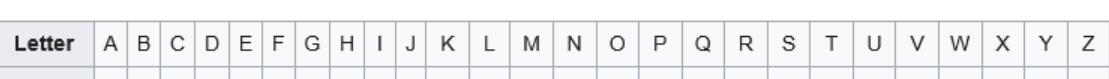
\includegraphics[width=121.38mm,height=21.68mm]{../../images/llm/page_009_img_01.png}%
\end{textblock*}

\end{document}
